\chapter{Recommentation System}\label{sec:rs}

\chapternote{Sequence-based Recommentation System}{Intern @ Tencent}

\begin{learningobjectives}
	\item Recommentation System
	\item Contrastive Learning
	\item Sequence Modeling
	\item Graph Neural Network
\end{learningobjectives}

\dependencies{NLP Basic}

\section{Contrastive Self-supervised Learning}

\concept{Self-supervised Learning}: a learning paradigm which aims to capture the intrinsic patterns and properties of input
data without using human-provided labels. For example, the two objectives of BERT.

\concept{Contrastive Self-supervised Learning}: generate (large number of) augmented examples of original data examples, create a task to predict whether two augmented examples come from the same original data example or not.
In CV, the augmentation includes cropping, flipping, distortion and rotation.
In NLP, it includes word deletion, reordering, and substitution.

SimCLR~\mycite{SimCLR}: $\boldsymbol{z}$ is a latent representation of the input image $\boldsymbol{x}$. Given a similar pair $(\boldsymbol{x}_i, \boldsymbol{x}_j)$, and a set of negative images $\boldsymbol{x}_k$ that dissimilar from the original image of $\boldsymbol{x}_i$, the contrastive loss is:

\begin{equation} \label{eq:simclr}
	- \log \frac{\exp(\text{sim}(\boldsymbol{z}_i, \boldsymbol{z}_j)/\tau)}{\exp(\text{sim}(\boldsymbol{z}_i, \boldsymbol{z}_j)/\tau) + \sum_k \exp(\text{sim}(\boldsymbol{z}_i, \boldsymbol{z}_k)/\tau)}
\end{equation}
where $\tau$ is a temperature parameter.

But SimCLR requires a large minibatch size to yield high performance.
MoCo (Momentum Contrast)~\mycite{MoCo} addresses this problem w/ the hypothesis that good features can be learned by a \emph{large} dictionary (by a queue) that covers a rich set of negative samples, while the encoder for the dictionary keys is kept as \emph{consistent} as possible (by momentum update) despite its evolution.
The queue contains many mini-batches.
In each step, the current mini-batch is enqueued to the dictionary queue, and the oldest mini-batch in the queue is removed.
To avoid rapidly changing encoder that reduces the key (i.e., the second parameter of $\text{sim}(\cdot, \cdot)$ in Eq.~\ref{eq:simclr}, and the first parameter is query) representations’ consistency.
The authors propose a momentum update ($\theta_k \leftarrow m\theta_k + (1 - m) \theta_q$ where $m$ is a large momentum coefficient, e.g., $0.99$, $\theta_q$ is parameters of the representation model of the query) to address this issue.
MoCo uses \emph{dual-encoder} architecture, i.e., a encoder $f_q$ for the query, and another encoder $f_k$ for keys.

CERT (Contrastive Self-supervised Learning for Language Understanding)~\mycite{fang2020cert} utilizes MoCo to fine-tune (aka., secondary pre-train) pre-trained BERT (or any other pre-training models).
The augmentation approach is \emph{back-translation}: given sentence $x$ of source language $S$, translate $x$ to $y$ in language $T$, and then translate $y$ back to augmented sample $x^\prime$ in language $S$.
With different $T$ and different translation model, we can collect many augmented samples.
However, the results of CERT are not significant and worse than ALBERT.

\begin{figure}[!thp]
	\centerline{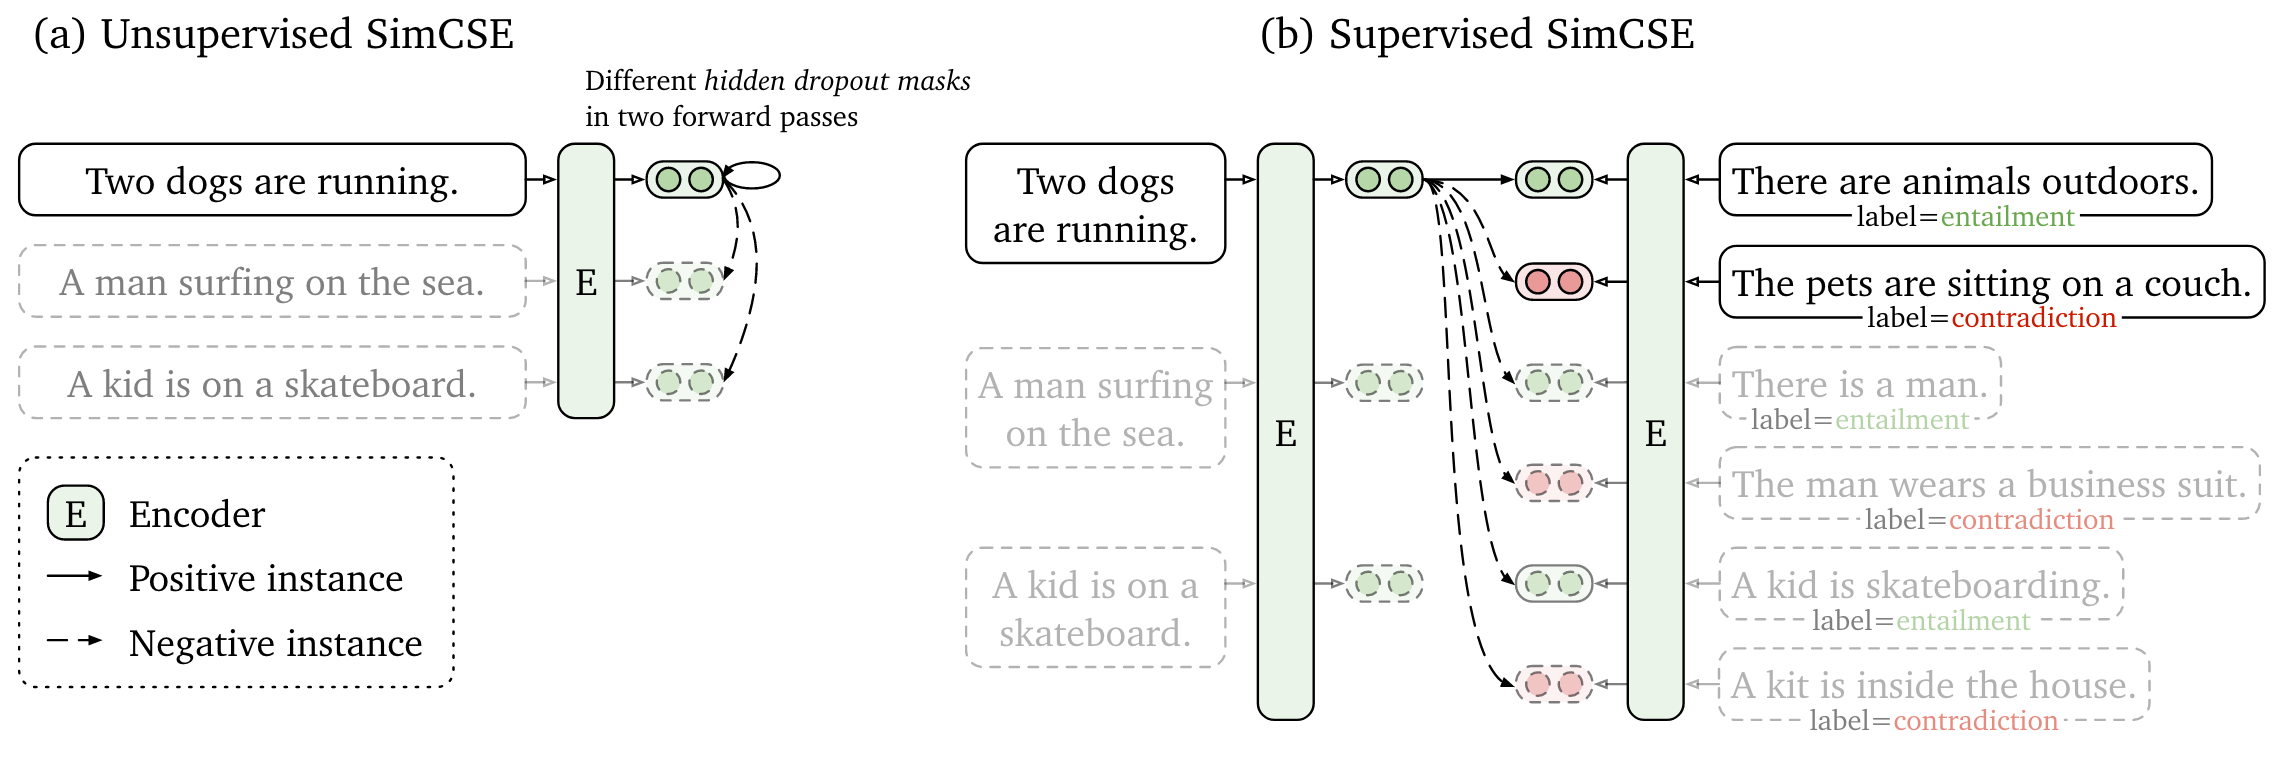
\includegraphics[width=10.0cm]{figs/SimCSE.png}}
	\caption{General idea of SimCSE.}
	\label{fig:SimCSE}
\end{figure}

SimCSE~\mycite{gao2021simcse} (Simple Contrastive Learning of Sentence Embeddings) leverages the dropout mask (like in BERT) to achieve the positve sample pairs, and proposes a supervised SimCSE w/ a natural language inference (NLI) datasets.
In the dataset, each sentence (aka., query) contains one entailment and one contradication.
The entailment is the positive sample (aka., key), the contradiction is the negative sample (key).
According to Want et al.~\mycite{wang2020hypersphere}, the quality of contrastive learning can be measured by alignment (the distance of the latent representations of the positive pair should close) and uniformity (the distance of the query and all the negative keys should scatter uniformly on the hypersphere).
It's shown~\mycite{wang2020hypersphere} that the anisotropy problem appears in language representations.
The number of (dominating and significant) singular values of the word embedding matrix in a language model decay drastically.
This is unfavorable to the uniformity.

ELECTRA~\mycite{clark2020electra} utilizes a GAN-style training process to learn a more powerful LM.
It uses MLM (masked language modeling, e.g., BERT) as the generator.
The output of the generator replaces the masked tokens with the predicted ones.
The discriminator is also a transformer encoder, whose \emph{replaced token detection} task is to predict whether each token in the output of generator is replaced by the generator or not.
The discriminator is the final pre-trained LM and the generator is a auxiliary network.
Compared with MLM-based methods, ELECTRA substantially outperforms them with less computations.
COCO-LM~\mycite{meng2021cocolm} enhances the replaced token detection of ELECTRA with CLM (Correcting Language Modeling).
The CLM is with a multi-task setting that combines the copy mechanism (aka., replaced token detection) and (a harder task) correction of the replaced tokens.
Pretraining at token level does not explicitly learn language semantics at the sequence level.
In addition to the token level pretraining, COCO-LM also introduces a sequence contrastive learning task (SCL).
The SCL is just a vanilla contractive learning where the query is the original sequence and the positive key is the randomly cropping of the query.
The output of \texttt{[CLS]} token is used as the representation of the whole sequence.

DeCLUTR~\mycite{DeCLUTR} proposes a token-level contrastive learning task based on span sampling.
The anchor is a randomly sampled span in a document.
For each anchor, there are multiple positive spans sampled near by the anchor.
The length of the anchor is longer than it's positives.
In most cases, the positive span is overlapped or subsumed with the anchor.
The negative spans inlcude easy (sampled from other documents) and hard negatives (sampled from the same document of the anchor).
A pooler (aka., mean pooling) maps the encodings of the tokens in the sample into a fixed-length encoding.
The performance of the mean pooling outperforms the embedding of \texttt{[CLS]} token.


\subsection{Relation to Metric Learning}

Metric learning is a type of representation learning that aims to learn an embedding space where the vector representations of similar data are mapped close together, and vice versa.
As a most successful approach of deep metric learning, contrastive learning attempts to close the distance between the anchor (aka., query) data point and some corresponding positive data points.
Under the setting of metric learning, MLM can be seen as an instance of contrastive learning.

\section{Graph Neural Networks}

